\documentclass[final]{beamer}

% ============================================================================
% 1. FORMATO GENERAL
% ============================================================================
% beamerposter permite conservar el requisito de la Escuela: A0 vertical.
% IEEEtran no se usa como clase porque esta diseñada para articulos, no para
% posters. Las convenciones IEEE se aplican a la estructura y las referencias.
\usepackage[orientation=portrait,size=a0,scale=1.0]{beamerposter}
\setbeamersize{text margin left=2cm,text margin right=2cm}
\usepackage[T1]{fontenc}
\usepackage[utf8]{inputenc}
\usepackage[spanish,es-tabla]{babel}
\usepackage{newtxtext,newtxmath}
\usepackage{microtype}
\usepackage{ragged2e}
\usepackage{booktabs}
\usepackage{tabularx}
\usepackage{array}
\usepackage{tikz}
\usetikzlibrary{arrows.meta,positioning,calc}
\usepackage{url}
\usepackage{cite}
\usepackage{graphicx}

\setbeamertemplate{navigation symbols}{}
\setbeamertemplate{bibliography item}{\insertbiblabel}
\urlstyle{same}

% ============================================================================
% 2. PALETA Y TIPOGRAFIA
% ============================================================================
\definecolor{Navy}{HTML}{000000}
\definecolor{IEEEBlue}{HTML}{000000}
\definecolor{BrightBlue}{HTML}{000000}
\definecolor{Teal}{HTML}{000000}
\definecolor{PaleBlue}{HTML}{FFFFFF}
\definecolor{PaleTeal}{HTML}{FFFFFF}
\definecolor{PaleGray}{HTML}{F2F2F2}
\definecolor{Coral}{HTML}{000000}
\definecolor{BodyText}{HTML}{000000}
\definecolor{RuleGray}{HTML}{777777}
\definecolor{White}{HTML}{FFFFFF}

\setbeamercolor{normal text}{fg=BodyText,bg=White}
\setbeamercolor{headline}{fg=Navy,bg=White}
\setbeamercolor{block title}{fg=BodyText,bg=White}
\setbeamercolor{block body}{fg=BodyText,bg=White}
\setbeamercolor{alerted text}{fg=Coral}
\setbeamercolor{trace}{fg=Navy,bg=White}
\setbeamercolor{finding number}{fg=White,bg=Coral}
\setbeamercolor{conclusion}{fg=BodyText,bg=White}
\setbeamercolor{repository}{fg=BodyText,bg=White}
\setbeamercolor{note}{fg=BodyText,bg=White}
\setbeamercolor{structure}{fg=BodyText}
\AtBeginDocument{\hypersetup{allcolors=black}}

\setbeamerfont{normal text}{size=\fontsize{31}{35}\selectfont}
\setbeamerfont{block title}{series=\mdseries,shape=\scshape,size=\fontsize{35}{39}\selectfont}
\setbeamerfont{block body}{size=\fontsize{31}{35}\selectfont}
\setlength{\parindent}{1.15em}
\setlength{\parskip}{0.08em}

% Encabezados de seccion centrados y sin relleno, como en el articulo IEEE
% usado como referencia visual.
\setbeamertemplate{block begin}{
  \vskip0.55cm
  \begin{beamercolorbox}[
    wd=\linewidth,
    sep=0.08cm,
    center
  ]{block title}
    \usebeamerfont{block title}\MakeUppercase{\insertblocktitle}
  \end{beamercolorbox}
  \vspace{0.28cm}
  \begin{beamercolorbox}[
    wd=\linewidth,
    sep=0cm
  ]{block body}
    \usebeamerfont{block body}\justifying
}
\setbeamertemplate{block end}{
  \end{beamercolorbox}
  \vskip0.25cm
}

% ============================================================================
% 3. COMANDOS REUTILIZABLES
% ============================================================================
\newcommand{\metric}[3][BrightBlue]{%
  \begin{minipage}[t]{0.47\linewidth}
    {\color{#1}\bfseries\fontsize{48}{51}\selectfont #2\par}
    \vspace{0.15cm}
    {\bfseries\fontsize{24}{28}\selectfont #3\par}
  \end{minipage}%
}

\newcommand{\finding}[3]{%
  \noindent
  {\bfseries\itshape #1) #2.}\enspace
  {\fontsize{27}{31}\selectfont #3\par}
  \vspace{0.40cm}
}

\newcommand{\smalltext}{\fontsize{25}{29}\selectfont}
\newcommand{\bodytext}{\fontsize{31}{35}\selectfont}
\newcommand{\posterfigcaption}[1]{%
  \vspace{0.18cm}
  {\fontsize{20}{24}\selectfont\justifying #1\par}
  \vspace{0.20cm}
}

% ============================================================================
% 4. DATOS DEL POSTER
% ============================================================================
\title{Diseño arquitectónico mínimo para sistemas RAG observables en español latinoamericano}
\author{Nicole Tatiana Parra Valverde}
\institute{Trabajo independiente}
\date{Segunda Escuela Sudamericana de NLP -- Sesión 2, orden 12}

\begin{document}
\begin{frame}[t]
\vspace*{1.90cm}

% ============================================================================
% 5. ENCABEZADO
% ============================================================================
\begin{beamercolorbox}[wd=\textwidth,sep=0cm]{headline}
  \centering
  {\color{BodyText}\scshape\fontsize{20}{24}\selectfont
    Segunda Escuela Sudamericana de NLP -- Buenos Aires -- 2026\par}
  \vspace{0.30cm}
  {\color{BodyText}\mdseries\fontsize{74}{80}\selectfont
    Diseño arquitectónico mínimo para sistemas RAG observables en español latinoamericano\par}
  \vspace{0.35cm}
  {\color{BodyText}\fontsize{29}{34}\selectfont
    Nicole Tatiana Parra Valverde\par}
  \vspace{0.10cm}
  {\color{BodyText}\itshape\fontsize{23}{28}\selectfont
    Trabajo independiente\par}
  \vspace{0.10cm}
  {\color{BodyText}\fontsize{21}{25}\selectfont
    Caso de estudio: normativa estudiantil del Tecnológico de Costa Rica\par}
\end{beamercolorbox}

\vspace{0.35cm}
\noindent{\color{BodyText}\rule{\textwidth}{0.045cm}}
\vspace{0.30cm}

% ============================================================================
% 6. CUERPO EN DOS COLUMNAS Y FIGURAS DE ARQUITECTURA
% ============================================================================
\begin{columns}[T,totalwidth=\textwidth]

% --------------------------------------------------------------------------
% COLUMNA 1: INDEXACION, INTRODUCCION, CORPUS Y METODO
% --------------------------------------------------------------------------
\begin{column}{0.485\textwidth}

\centering
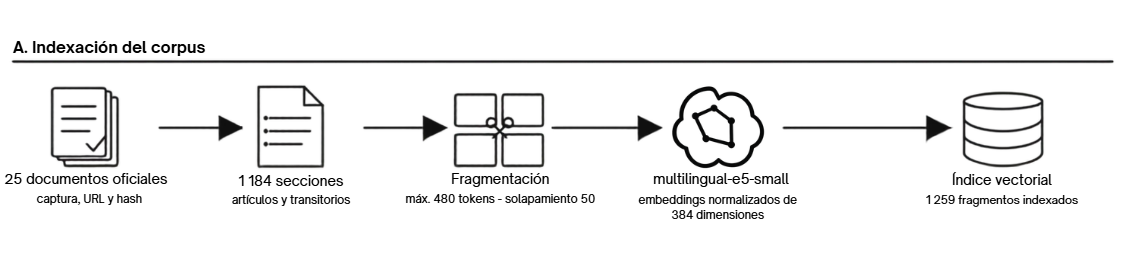
\includegraphics[
  width=0.99\linewidth
]{figures/figura-a-indexacion-corpus}
\posterfigcaption{\textbf{Fig. 1.} Flujo de indexación del corpus. Los
documentos oficiales se transforman en secciones, fragmentos y embeddings
normalizados antes de construir el índice vectorial local.}

\begin{block}{I. Introducción}
\noindent\textbf{\textit{Resumen---}}La generación aumentada por recuperación
(RAG) incorpora evidencia externa al contexto de un modelo de lenguaje
\cite{lewis2020rag}. Sin embargo, una respuesta final no permite establecer por
sí sola si un fallo se originó en la recuperación, la generación o la
validación. Este trabajo presenta una arquitectura RAG mínima, local y
reproducible para normativa en español latinoamericano. El diseño conserva una
traza por consulta y expone los artefactos necesarios para auditar cada
resultado.

\vspace{0.30cm}
\noindent\textbf{\textit{Contribución---}}Se implementó un pipeline
reproducible que integra indexación documental, recuperación semántica,
generación local, validación de citas y observabilidad básica, sin depender de
una plataforma de despliegue compleja.

\vspace{0.30cm}
{\smalltext\noindent\textbf{\textit{Palabras clave---}}RAG, PLN en español,
recuperación de información, observabilidad, modelos de lenguaje.}
\end{block}

\begin{block}{II. Corpus e indexación}
\begin{columns}[T,totalwidth=\linewidth]
  \begin{column}{0.30\linewidth}
    {\color{Teal}\bfseries\fontsize{42}{45}\selectfont 25\par}
    {\bfseries\smalltext documentos oficiales}
  \end{column}
  \begin{column}{0.34\linewidth}
    {\color{Teal}\bfseries\fontsize{42}{45}\selectfont 1\,184\par}
    {\bfseries\smalltext secciones procesadas}
  \end{column}
  \begin{column}{0.32\linewidth}
    {\color{Teal}\bfseries\fontsize{42}{45}\selectfont 1\,259\par}
    {\bfseries\smalltext fragmentos indexados}
  \end{column}
\end{columns}

\vspace{0.55cm}
El caso de estudio comprende normativa estudiantil publicada por el
Tecnológico de Costa Rica. Cada captura conserva la URL oficial, la fecha de
recolección y una suma SHA-256. El procesamiento produjo 1\,141 artículos y 43
disposiciones transitorias. Las secciones de mayor longitud se dividieron con
un máximo de 480 tokens y un solapamiento de 50, lo que generó 1\,259
fragmentos indexados. El corpus, sus metadatos y el procesamiento se
versionaron en el repositorio \cite{tec2026reglamentos}. La Fig. 1 resume esta
ruta de transformación.
\end{block}

\begin{block}{III. Diseño e implementación}
Los fragmentos se codificaron con
\texttt{intfloat/multilingual-e5-small} \cite{wang2024e5}. Cada representación
contiene 384 dimensiones y se normalizó antes de almacenarse. Durante la
consulta, el orquestador codifica la pregunta, calcula la similitud coseno
contra el índice y recupera los cinco fragmentos con mayor puntuación.

\vspace{0.35cm}
El contexto recuperado y la pregunta se envían a Qwen3.5:9B mediante Ollama.
La generación se ejecuta localmente con temperatura 0,1 y un contrato JSON que
limita el estado a \texttt{answered} o \texttt{not\_found}. Una validación
posterior comprueba el estado, el texto y los identificadores de cita antes de
presentar la respuesta.

\vspace{0.35cm}
\noindent{\bfseries\smalltext
Configuración principal: top-5; similitud coseno; Qwen3.5:9B Q4\_K\_M;
temperatura 0,1; ejecución local.}
\end{block}

\begin{block}{IV. Protocolo de evaluación}
La evaluación utilizó 40 preguntas de referencia: 25 directas, 8 que requieren
evidencia de varias secciones y 7 no respondibles con el corpus. Para cada
consulta se conservaron los fragmentos recuperados, sus puntuaciones, el
contexto, la respuesta, el estado, las citas y los tiempos.

\vspace{0.35cm}
Las respuestas se revisaron manualmente con seis criterios: corrección factual,
cobertura, fidelidad a las fuentes, claridad, presencia de evidencia de
referencia y conclusión global. Las métricas automáticas se utilizaron para
describir recuperación, citas y latencia; no se interpretaron como una medida
de exactitud factual.
\end{block}

\begin{block}{V. Observabilidad por consulta}
Como muestra la Fig. 2, cada ejecución válida produce un registro JSON con
cuatro grupos de información.
\textit{Configuración} identifica el corpus, el índice, los modelos y sus
parámetros. \textit{Recuperación} conserva los fragmentos, los identificadores,
el orden, las puntuaciones y la procedencia oficial. \textit{Generación}
registra latencia, tokens y características del contexto. \textit{Resultado}
incluye el estado, la respuesta, las citas validadas y las fuentes citadas.

\vspace{0.35cm}
La traza se utiliza como un artefacto diagnóstico, no como una métrica de
calidad. Su propósito es atribuir un fallo a la etapa que lo produjo y permitir
que una ejecución pueda examinarse posteriormente sin repetirla.
\end{block}

\begin{block}{Código, datos y documentación}
\centering
{\smalltext Repositorio reproducible:\par}
\vspace{0.15cm}
{\bfseries\fontsize{25}{29}\selectfont
\url{https://github.com/niparra21/nlpArgentina}}
\end{block}

\end{column}

% --------------------------------------------------------------------------
% COLUMNA 2: CONSULTA, RESULTADOS, DISCUSION Y CONCLUSION
% --------------------------------------------------------------------------
\begin{column}{0.485\textwidth}

\centering
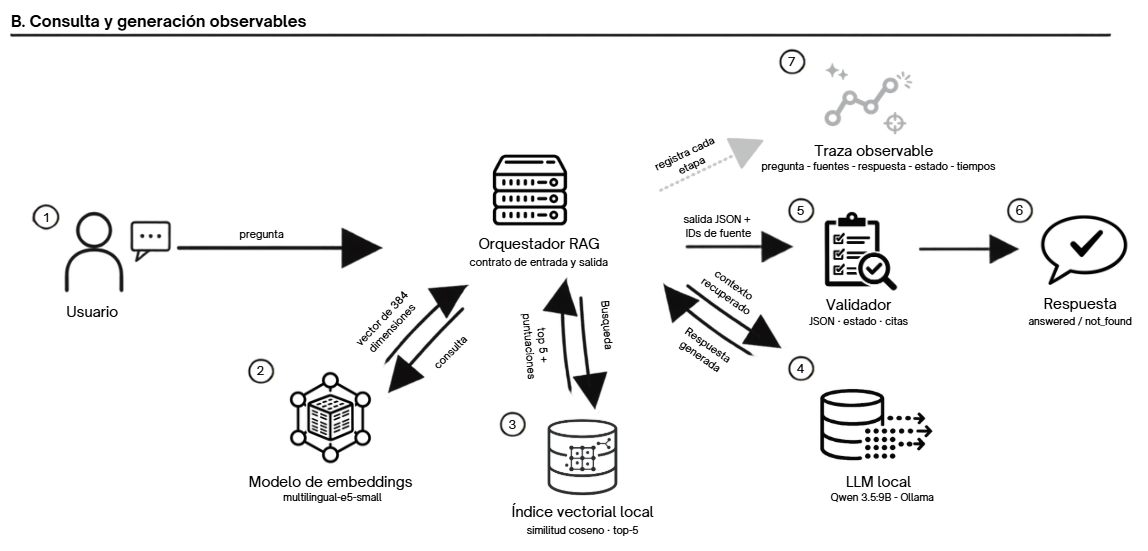
\includegraphics[
  width=0.99\linewidth
]{figures/figura-b-consulta-observable}
\posterfigcaption{\textbf{Fig. 2.} Flujo de consulta y generación observables.
El orquestador coordina embeddings, recuperación, generación y validación; la
traza conserva pregunta, fuentes, respuesta, estado y tiempos.}

\begin{block}{VI. Resultados}
\begin{center}
  {\fontsize{22}{26}\selectfont\textsc{Tabla I}\par}
  {\fontsize{21}{25}\selectfont\textsc{Resultados cuantitativos del
  prototipo}\par}
\end{center}

\vspace{0.20cm}
{\fontsize{21}{25}\selectfont
\renewcommand{\arraystretch}{1.14}
\begin{tabularx}{\linewidth}{
  @{}
  >{\raggedright\arraybackslash}X
  >{\centering\arraybackslash}p{4.8cm}
  >{\raggedleft\arraybackslash}p{4.4cm}
  @{}
}
\toprule
\textbf{Indicador} & \textbf{Casos} & \textbf{Resultado} \\
\midrule
\multicolumn{3}{@{}l}{\textit{Evaluación automática}} \\
Salidas estructuralmente válidas & 37/40 & 92,5\,\% \\
Decisión de estado correcta & 35/40 & 87,5\,\% \\
Evidencia de referencia en top-5 & 31/33 & 93,9\,\% \\
Al menos una cita de referencia & 27/33 & 81,8\,\% \\
Toda la evidencia esperada citada & 25/33 & 75,8\,\% \\
Abstención en no respondibles & 7/7 & 100\,\% \\
\addlinespace[0.16cm]
\multicolumn{3}{@{}l}{\textit{Revisión humana}} \\
Corrección factual estricta & 26/33 & 78,8\,\% \\
Puntaje factual ponderado & 28,5/33 & 86,4\,\% \\
Fidelidad total a fuentes & 29/31 & 93,5\,\% \\
Cobertura completa & 24/33 & 72,7\,\% \\
Conclusión aprobada & 28/40 & 70,0\,\% \\
\addlinespace[0.16cm]
\multicolumn{3}{@{}l}{\textit{Latencia promedio}} \\
Búsqueda semántica & 40 consultas & 27 ms \\
Generación local & 37 salidas & 5,36 s \\
Pipeline completo & 40 consultas & 5,53 s \\
\bottomrule
\end{tabularx}
}

\vspace{0.28cm}
{\fontsize{20}{24}\selectfont\justifying
\textit{Nota:} Las métricas de recuperación y citas utilizan las 33 preguntas
respondibles. La fidelidad excluye nueve casos sin afirmaciones evaluables. La
generación concentró la mayor parte de la latencia total.\par}

\vspace{0.45cm}
\centering
{\fontsize{21}{25}\selectfont\textit{Aprobación manual por tipo de pregunta}\par}
\vspace{0.10cm}
\centering
\begin{tikzpicture}[x=0.060\linewidth,y=1.44cm]
  \draw[draw=RuleGray,line width=1.2pt] (0,0) -- (10,0);
  \foreach \x/\label in {0/0,2/20,4/40,6/60,8/80,10/100} {
    \draw[draw=RuleGray] (\x,0.05) -- (\x,-0.08);
    \node[below,font=\fontsize{18}{21}\selectfont,text=BodyText]
      at (\x,-0.08) {\label\%};
  }

  \node[left,align=right,text width=6.0cm,
    font=\fontsize{19}{22}\selectfont,text=BodyText]
    at (0,1.2) {Directas · 19/25};
  \fill[BrightBlue] (0,0.84) rectangle (7.6,1.50);
  \node[right,font=\bfseries\fontsize{19}{22}\selectfont,text=Navy]
    at (7.6,1.17) {76\%};

  \node[left,align=right,text width=6.0cm,
    font=\fontsize{19}{22}\selectfont,text=BodyText]
    at (0,2.30) {Varias secciones · 2/8};
  \fill[BrightBlue] (0,1.94) rectangle (2.5,2.60);
  \node[right,font=\bfseries\fontsize{19}{22}\selectfont,text=Navy]
    at (2.5,2.27) {25\%};

  \node[left,align=right,text width=6.0cm,
    font=\fontsize{19}{22}\selectfont,text=BodyText]
    at (0,3.40) {No respondibles · 7/7};
  \fill[BrightBlue] (0,3.04) rectangle (10,3.70);
  \node[left,font=\bfseries\fontsize{19}{22}\selectfont,text=White]
    at (9.85,3.37) {100\%};
\end{tikzpicture}

\vspace{0.35cm}
\justifying
El sistema resolvió mejor las preguntas directas y las abstenciones. La menor
aprobación en preguntas multisección indica que la presencia de alguna
evidencia pertinente no garantiza cobertura completa.
\end{block}

\begin{block}{VII. Discusión: valor de la observabilidad}
\finding{1}{Evidencia distribuida}{
  Solo 2 de 8 preguntas multisección fueron aprobadas. En varios casos se
  recuperó una parte de la evidencia, pero no todos los artículos necesarios.}

\finding{2}{Documento correcto, fragmento incorrecto}{
  En q029 se recuperó el artículo relacionado, pero no el fragmento que
  contenía el dato. Una evaluación limitada al documento habría ocultado el
  fallo.}

\finding{3}{Contenido correcto, salida inválida}{
  q025 y q032 se rechazaron porque las citas visibles y estructuradas no
  coincidían. La validez del contrato de salida constituye una dimensión
  adicional de calidad.}

\finding{4}{Abstención confiable}{
  Las siete preguntas sobre información ausente recibieron
  \texttt{not\_found}, sin producir afirmaciones no respaldadas.}
\end{block}

\begin{block}{VIII. Limitaciones y trabajo futuro}
El estudio utiliza un único dominio documental, un modelo de embeddings, un
modelo generativo, 40 preguntas y una persona revisora. Tampoco compara
recuperación léxica, híbrida o con reranking; por tanto, los resultados no
representan toda la diversidad del español latinoamericano.

\vspace{0.35cm}
El trabajo futuro evaluará reranking para evidencia multisección, recuperación
densa frente a alternativas léxicas e híbridas, nuevos dominios y países, y
umbrales de abstención con revisión humana adicional.
\end{block}

\begin{block}{IX. Conclusión}
\noindent{\bfseries
Una arquitectura RAG pequeña puede proporcionar trazabilidad útil sin requerir
una plataforma de observabilidad compleja.}

\vspace{0.35cm}
La conservación de evidencia, citas, estados y tiempos permitió diferenciar
fallos de recuperación, generación y validación. El principal reto no fue la
abstención, sino la cobertura de evidencia distribuida. En consecuencia, una
arquitectura observable debe distinguir documentos de fragmentos y validar la
consistencia de las citas antes de entregar la respuesta.
\end{block}

\end{column}
\end{columns}

\vspace{0.45cm}

% ============================================================================
% 7. REFERENCIAS IEEE Y PIE
% ============================================================================
\begin{beamercolorbox}[wd=\textwidth,sep=0cm]{block body}
  {\color{Navy}\bfseries\fontsize{26}{30}\selectfont X. Referencias\par}
  \vspace{0.25cm}
  {\fontsize{18}{22}\selectfont
    \bibliographystyle{IEEEtran}
    \bibliography{references}
  }
\end{beamercolorbox}

\vspace{0.10cm}
\begin{columns}[T,totalwidth=\textwidth]
  \begin{column}{0.76\textwidth}
    {\color{BodyText}\fontsize{18}{22}\selectfont
      Los resultados corresponden a una corrida reproducible del prototipo y
      no sustituyen la consulta de la normativa oficial.}
  \end{column}
  \begin{column}{0.22\textwidth}
    \raggedleft
    {\color{Navy}\bfseries\fontsize{18}{21}\selectfont Sesión 2 · Orden 12}
  \end{column}
\end{columns}

\end{frame}
\end{document}
